\documentclass[11pt,a4paper]{ctexart}

\usepackage[margin=2.6cm]{geometry}
\usepackage{amsmath,amssymb,amsthm}
\usepackage{graphicx}
\usepackage{booktabs}
\usepackage{hyperref}
\usepackage{xcolor}
\usepackage{listings}
\usepackage{caption}

\graphicspath{{figures/}}
\hypersetup{colorlinks=true, linkcolor=blue!50!black, urlcolor=blue!60!black}
\lstset{
  basicstyle=\ttfamily\small,
  breaklines=true,
  frame=single,
  columns=fullflexible,
  backgroundcolor=\color{gray!7}
}

\newtheorem{definition}{定义}[section]
\newtheorem{theorem}{定理}[section]
\newtheorem{lemma}{引理}[section]
\newtheorem{proposition}{命题}[section]
\newtheorem{example}{例}[section]

\title{第 13 章 \quad Nonlinear Time Series Models / 非线性时间序列模型}
\author{基于 \textit{A Course in Time Series Analysis} 的中文讲义与 Python 实践}
\date{}

\begin{document}
\maketitle

\section*{本章学习目标}

本章按照原文 \textit{Nonlinear Time Series Models} 的小节顺序整理，保留主要定义、定理、模型公式和练习方向，并将原文中的 R 实践思路改写为 Python 工程实践。

完成本章后，应能够：
\begin{itemize}
  \item 理解非线性递推模型的平稳解条件；
  \item 用金融数据动机说明波动聚集；
  \item 掌握 ARCH、GARCH、IGARCH 模型；
  \item 理解双线性模型和随机系数 AR；
  \item 了解非参数时间序列模型。
\end{itemize}

\section{非线性模型的一般形式}

原文以随机递推方程为入口：
\[
  X_t=F(X_{t-1},\varepsilon_t).
\]
\begin{theorem}[Brandt 定理，原文 Theorem 13.0.1]
在随机映射满足平均收缩等条件时，上述递推存在唯一严格平稳解，并可由过去创新的可测函数表示。
\end{theorem}

该定理为 ARCH、GARCH 和双线性模型的存在性提供统一思路。

\section{数据动机}

金融收益序列常呈现三个特征：收益均值相关弱、平方收益或绝对收益相关强、波动成团出现。线性 ARMA 均值模型难以解释这种条件方差变化，因此需要非线性模型。

\section{ARCH 模型}

ARCH(p) 定义为
\[
  X_t=\sigma_t Z_t,\qquad
  \sigma_t^2=a_0+a_1X_{t-1}^2+\cdots+a_pX_{t-p}^2,
\]
其中 \(Z_t\) 通常为 iid 标准化创新。若 \(a_i\ge0\)，可保证条件方差非负。

\subsection{ARCH 的特征}

虽然 \(X_t\) 可不相关，但 \(X_t^2\) 相关，因此模型能刻画波动聚集。

\section{GARCH 模型}

GARCH(1,1) 为
\[
  X_t=\sigma_tZ_t,\qquad
  \sigma_t^2=a_0+a_1X_{t-1}^2+b_1\sigma_{t-1}^2.
\]
若 \(a_1+b_1<1\)，常见二阶平稳条件成立，且
\[
  E(X_t^2)=\frac{a_0}{1-a_1-b_1}.
\]

\begin{example}[GARCH(1,1) 反演，原文 Example 13.3.1]
当 \(b_1<1\) 时，\(\sigma_t^2\) 可展开为过去平方收益的无限加权和，权重按 \(b_1\) 衰减。
\end{example}

\begin{definition}[IGARCH，原文 Definition 13.3.1]
若 GARCH 模型满足 \(a_1+b_1=1\)，称为 IGARCH。此时波动冲击具有极强持续性。
\end{definition}

\section{双线性模型与非参数模型}

双线性模型包含过去观测和过去创新的乘积项，例如
\[
  X_t=\phi X_{t-1}+\theta\varepsilon_{t-1}
      +bX_{t-1}\varepsilon_{t-1}+\varepsilon_t.
\]
它比线性 ARMA 更灵活，可产生非线性依赖。

非参数时间序列模型则把条件均值或条件方差写成未知函数：
\[
  X_t=m(X_{t-1},\ldots,X_{t-p})+\varepsilon_t,
\]
再用核方法、局部线性、样条或机器学习方法估计 \(m\)。原文将其作为高级扩展。

\section{原文数据与模型补充}

\subsection{Yahoo 和 FTSE 数据动机}
原文第 13.1 节用 Yahoo 1996--2014 数据和 2014 年 1--8 月 FTSE 100 数据展示金融收益特征：价格序列非平稳，收益序列均值相关弱，但平方收益和绝对收益显示明显聚集。

\subsection{ARCH 的存在性和二阶平稳}
\begin{theorem}[ARCH 平稳性说明]
ARCH(p) 的严格平稳解可由随机递推理论给出；二阶平稳通常要求 ARCH 系数和小于 1。
\end{theorem}

\subsection{GARCH 扩展}
原文第 13.3.2 还提到 GARCH 的扩展形式，例如非对称 GARCH、EGARCH 或含外生变量的条件方差模型，用于刻画杠杆效应和更复杂的波动动态。

\subsection{R 代码与模拟练习}
第 13.3.3 和 13.4.3 给出 R 代码提示。Exercise 13.1 推导 GARCH 条件，Exercise 13.2 模拟 ARCH/GARCH，Exercise 13.3 模拟双线性模型，Exercise 13.4 研究随机系数 AR 模型。

\begin{example}[随机系数 AR]
随机系数 AR 可写为
\[
  X_t=(\phi+\eta_t)X_{t-1}+\varepsilon_t.
\]
即使条件均值类似 AR(1)，随机系数也会带来非线性依赖和时变波动。
\end{example}

\section{Python 工程实践}

在本章目录下运行：
\begin{lstlisting}[language=bash]
python scripts/ch13_generate_figures.py
\end{lstlisting}

脚本会把图像写入本章 \texttt{figures/} 目录。当前图像用于配合本章核心概念的仿真说明；若后续补齐原始数据文件，可把模拟数据替换为原文真实数据案例。

\begin{figure}[htbp]
  \centering
  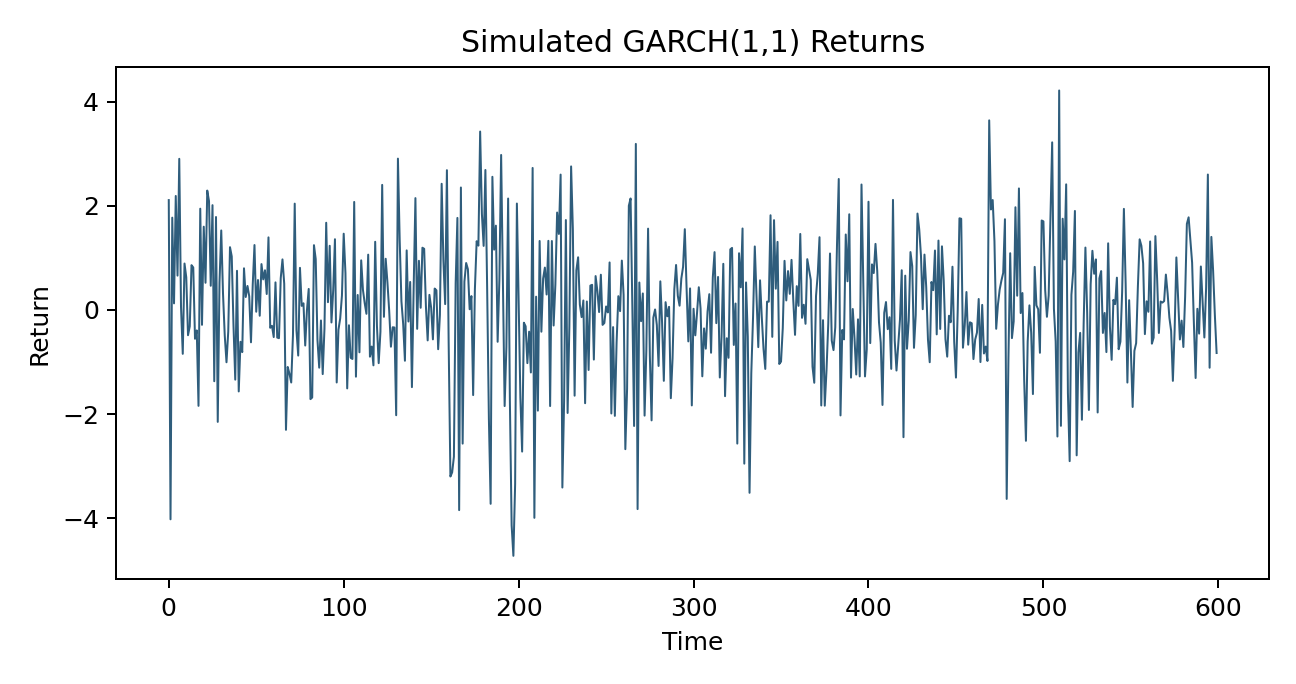
\includegraphics[width=0.86\textwidth]{ch13_fig01_garch_returns.png}
  \caption{GARCH(1,1) 收益模拟：收益本身均值稳定，但波动呈现聚集。}
\end{figure}

\begin{figure}[htbp]
  \centering
  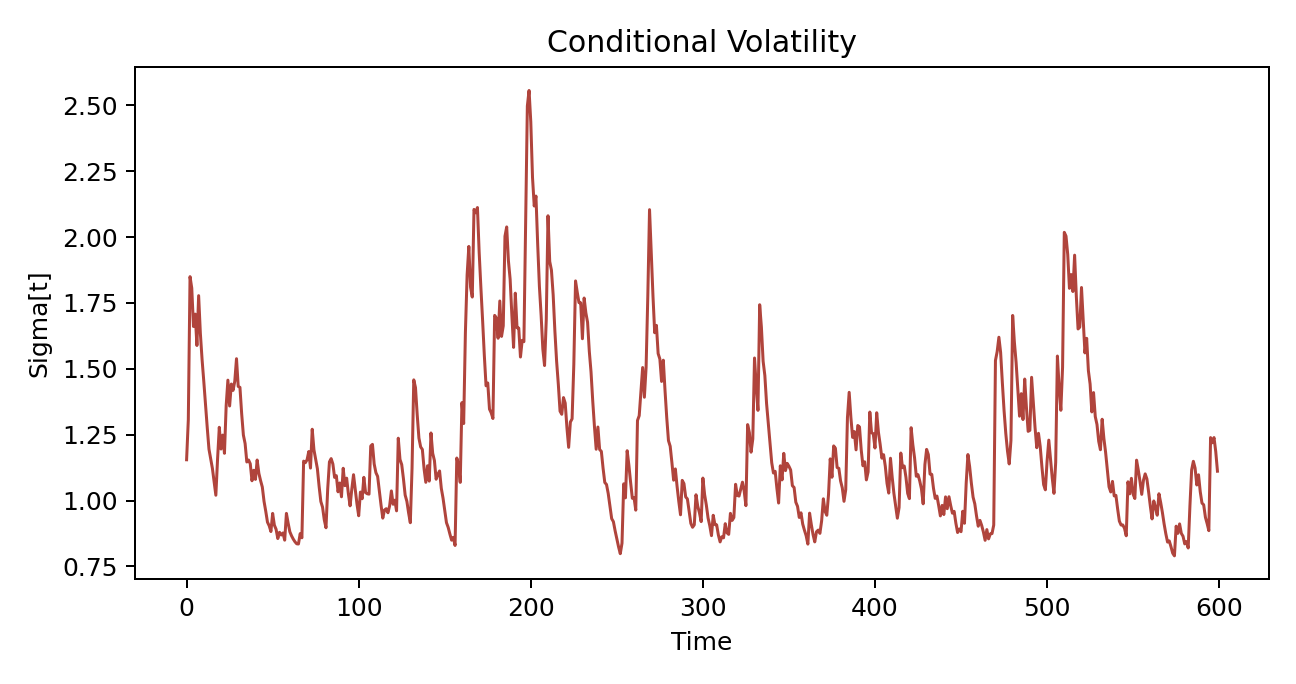
\includegraphics[width=0.86\textwidth]{ch13_fig02_conditional_volatility.png}
  \caption{条件波动率路径：GARCH 模型通过递推方差刻画风险随时间变化。}
\end{figure}

\section{练习提要}

原文练习主要围绕下列方向展开：
\begin{itemize}
  \item 推导 ARCH(1) 二阶平稳条件；
  \item 模拟 ARCH 与 GARCH 并比较 ACF 和平方 ACF；
  \item 分析 IGARCH 的持续性；
  \item 模拟双线性或随机系数 AR 模型。
\end{itemize}

\section*{本章小结}

第 13 章从线性均值模型转向条件方差和非线性依赖。ARCH/GARCH 解释金融数据的波动聚集，双线性和非参数模型则展示了更一般的非线性动态。

\end{document}
